\section{src/chord.cpp File Reference}
\label{chord_8cpp}\index{src/chord.\+cpp@{src/chord.\+cpp}}
{\ttfamily \#include \char`\"{}chord.\+h\char`\"{}}\newline
{\ttfamily \#include \char`\"{}langnotes.\+h\char`\"{}}\newline
{\ttfamily \#include \char`\"{}language.\+h\char`\"{}}\newline
{\ttfamily \#include \char`\"{}chordutil.\+h\char`\"{}}\newline
{\ttfamily \#include $<$Q\+Application$>$}\newline
{\ttfamily \#include $<$Q\+Reg\+Exp$>$}\newline
{\ttfamily \#include $<$Q\+Sql\+Query$>$}\newline
{\ttfamily \#include $<$Q\+Sql\+Error$>$}\newline
{\ttfamily \#include $<$Q\+String$>$}\newline
{\ttfamily \#include $<$Q\+String\+List$>$}\newline
{\ttfamily \#include $<$Q\+Variant$>$}\newline
{\ttfamily \#include $<$Q\+Debug$>$}\newline
{\ttfamily \#include $<$Q\+Settings$>$}\newline
Include dependency graph for chord.\+cpp\+:\nopagebreak
\begin{figure}[H]
\begin{center}
\leavevmode
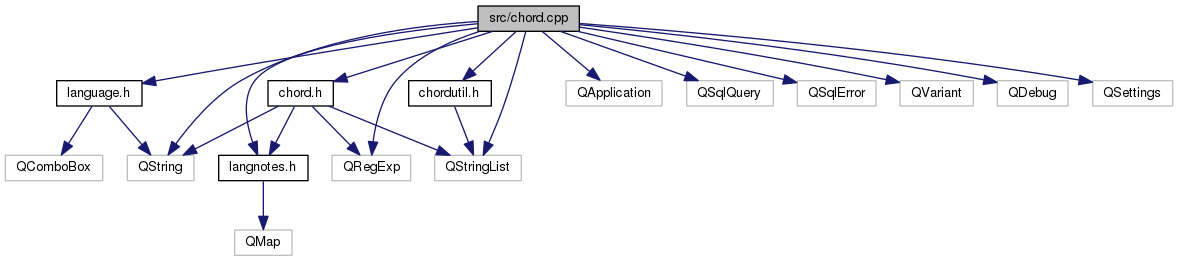
\includegraphics[width=350pt]{chord_8cpp__incl}
\end{center}
\end{figure}
